\chapter{Evaluation of results}


The hyperparameter optimization and model selection process was run on a number of datasets that
include 29 standard datasets commonly used in the machine learning community, and 8 datasets taken from
biological experiments. The datasets were also analyzed under the default settings for all SML
algorithms.

The SML algorithms applied on the datasets were:

\begin{tabularx}{\textwidth}{l l l}
\texttt{PassiveAggressive} &
\texttt{RadiusNeighbors} &
\texttt{GaussianNB} \\
\texttt{ExtraTreeEnsemble} &
\texttt{SVM} &
\texttt{LinearDiscriminant} \\
\texttt{KNN} &
\texttt{RandomForest} &
\texttt{StochasicGradientDescent} \\
\texttt{LogisticRegression} &
\texttt{NearestCentroid} & 
\texttt{LinearSVM}\\
\texttt{NuSVM} &
\texttt{DecisionTree} &
\texttt{Ridge} \\
\texttt{QuadraticDiscriminant} &
\texttt{GradientBoosting} &
\end{tabularx}


The optimization stage for each of the datasets was run during 8 hours as distributed tasks on the
Brutus Cluster.

A comparison between the performance indices obtained by using default and optimized hyperparameters
is show in table \ref{tb:comparison_all}.

In general, the performance indices of the optimized models are significantly higher than the
performance indices under the default configurations. A few datasets did not show improvement over
the default settings. In these cases, the best classification performance was obtained by using the
LinearDiscriminant classifier, which does not expose any hyperparameters to configure.

The table shows that the SML algorithm that performs best and improvement over the default settings
strictly depends on the dataset.

\begin{table}[h!]
\centering
\begin{tabularx}{\textwidth}{l r r r r r l}
	& \multicolumn{2}{c}{\bf default} & ~ & \multicolumn{3}{c}{\bf Optimized}\\
	\cline{2-3}
	\cline{5-7}
{\bf Dataset} & Worst & Best & ~ & Score & Boost & Family\\
	\cline{1-7}
	\input{images/comparison_table.txt}
\end{tabularx}
\caption{Comparison of optimized and default performance indices for all datasets.}
\label{tb:comparison_all}
\end{table}

\section{Results on standard Machine Learning datasets}

Standard datasets are commonly used for testing and evaluating machine learning approaches. Some of
the datasets used here are inherently difficult to classify, and hence most SML algorithms
consistently obtain a very low performance index; other datasets are simple to classify and hence
good performance indices but little relative improvement over the default values is expected.

Figure \ref{img:optvsdefstandard} shows an example of the distribution of performance indices for
different models, and their shift with respect to the performance indices obtained by the default
models, for a specific standard dataset. Each row in the plot corresponds to a different algorithm
under the default and optimized settings (thin and thick boxplots, respectively). Distributions that
are not significantly different from the best, up to a confidence level $\alpha$ shown on the title of the
plot, are highlighted in blue. The p-values reported by the statistical test are displayed on the right side
of the plot. Models with p-values above the $\alpha$ level are considered statistically
indistinguishable from one another.

The baseline is shown as a vertical dotted line. It is possible for some models to score lower than the
baseline, as explained in section \ref{sec:performance_measurement}.

In cases where algorithms do not work at all on a given dataset, their performance indices are
reported as a single point over the baseline.

\begin{figure}[t!]
	\centering
	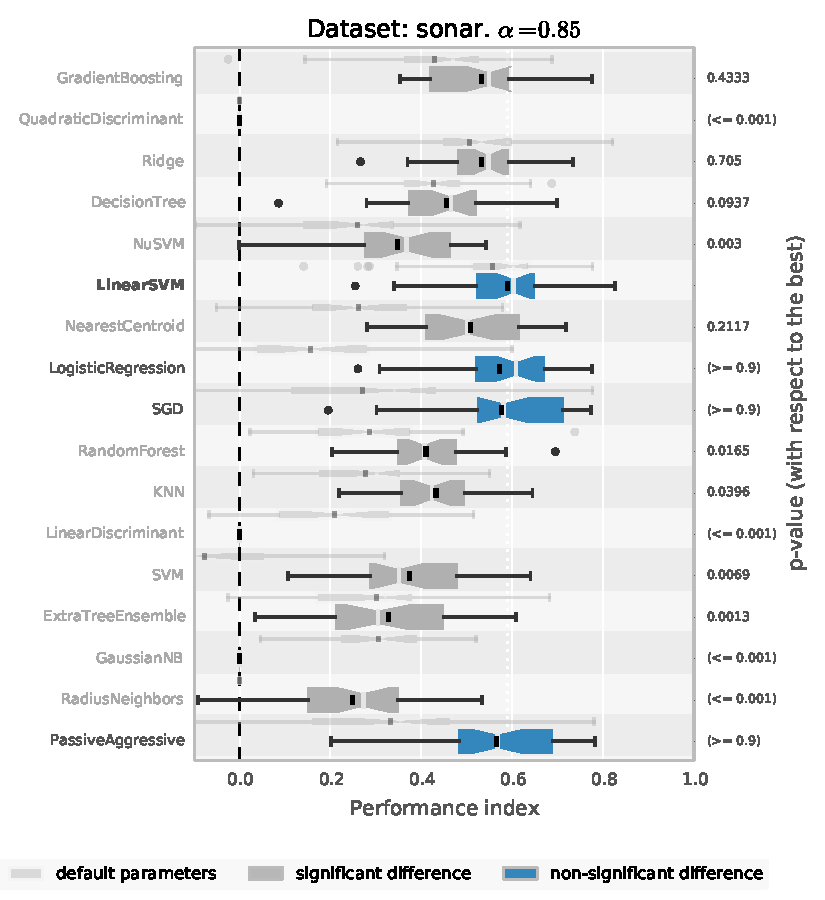
\includegraphics{optimized_vs_default_standard}
	\caption{Optimized vs default values for a standard machine learning dataset}
	\label{img:optvsdefstandard}
\end{figure}


\section{Results on biological data}

\begin{figure}[h!]
	\centering
	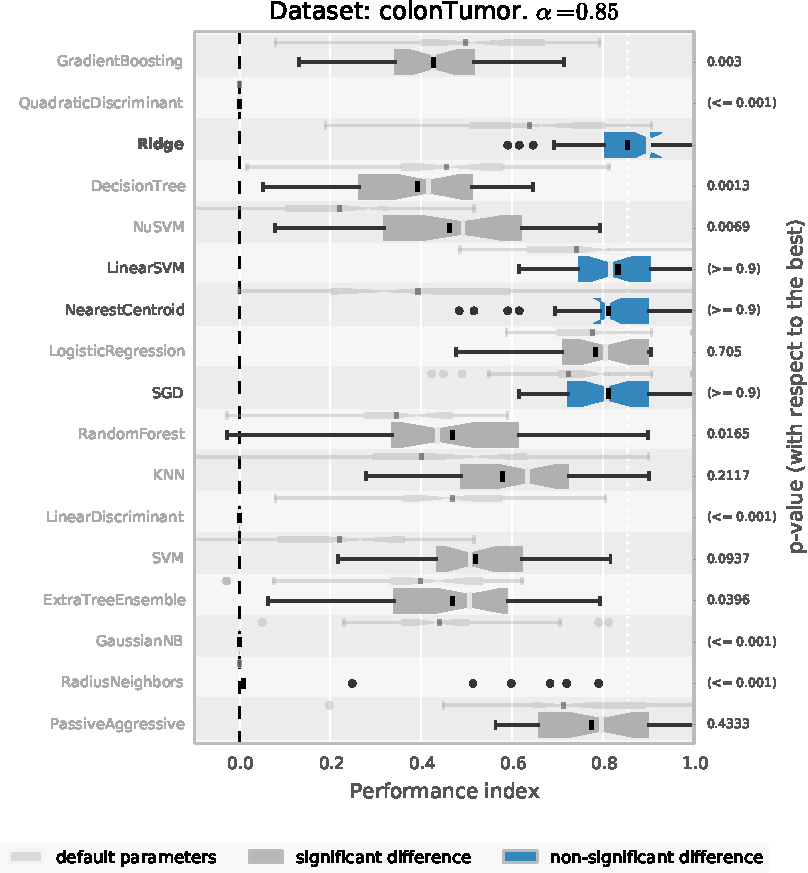
\includegraphics[width=.49\textwidth]{optimized_vs_default_bio1}
	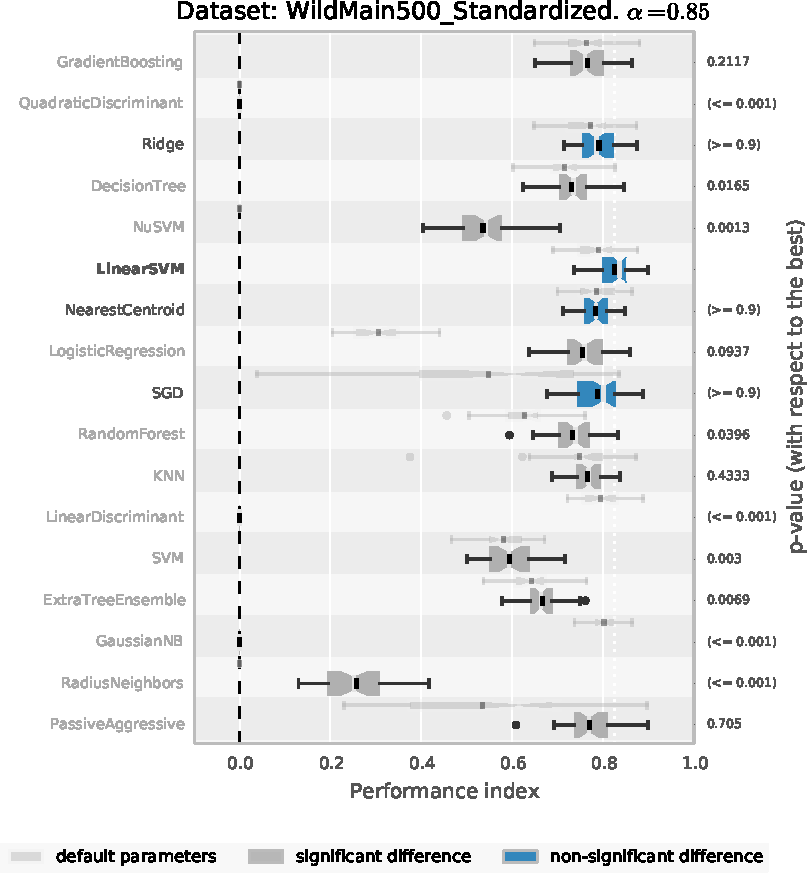
\includegraphics[width=.49\textwidth]{optimized_vs_default_bio2}
	\caption[Optimized vs default values for biological datasets of different sizes]{Optimized vs
	default values for biological datasets of different sizes. The colonTumor dataset contains 62
	instances, whereas the WildMain500\_Standarized dataset contains 500 instances.}
	\label{img:optvsdefbio}
\end{figure}

Similar results are obtained when the method is applied on biological datasets. Figure
\ref{img:optvsdefbio} shows the distribution of performance indices for different SML algorithms
applied on a small dataset (62 instances), and a larger dataset (500 instances). A large spread of
the scores is due precisely to the dataset size, as can be immediately noticed when comparing
both plots. The variance of the candidate models is in general
smaller than the variance of the performance indices from the default configuration. In particular,
the models statistically indistinguishable from the best exhibit a smaller variance than the rest,
since the stability of the performance index is one of the criteria considered for model selection.

\section{General prior learning}

The 29 standard machine learning datasets were used to learn general priors for all numerical
hyperparameters on all SML algorithms, as explained in \ref{sec:learning_prior}. 

The learned distributions encode the detected regions with good hyperparameter values. In many cases
there is no clear agreement on the regions where useful values of the hyperparameter lie, and hence
the learned distribution assigns relatively similar density to the whole hyperparameter domain.
Using such a learned prior is roughly equivalent to using a uniform distribution.

Since different combinations of categorical variables define different contexts that might change
the semantics of the numerical hyperparameter, general prior distributions are learned independently
for each categorical context.

As an example, we present the learned distributions of the hyperparameter $\gamma$ for two different
kernels used by a support vector machine classifier.

The distributions learned by analyzing the values of $\gamma$ for a polynomial kernel, shown in
Figure \ref{fig:learned_gamma1}, look similar, regardless of the value of other categorical
hyperparameters. Both distributions shown assign a rather uniform density over the entire (0,1)
domain, and no important improvement in the optimization process should be expected when such
distribution is used as a general prior.

Figure \ref{fig:learned_gamma2} shows the learned general prior for the same numerical
hyperparameter $\gamma$ when used with a sigmoid kernel. In this case, the evaluation of the
hyperparameter on the large group of datasets seems to usually achieve better performance when small
values (close to zero) are used, althought the assignment of values away from zero is also allowed.
This skewness of the learned distribution, when using a sigmoid kernel, may be used when looking for
optimal values of $\gamma$ on other datasets, as a suggestion of where to look first.

\begin{figure}[h!]
	\centering
	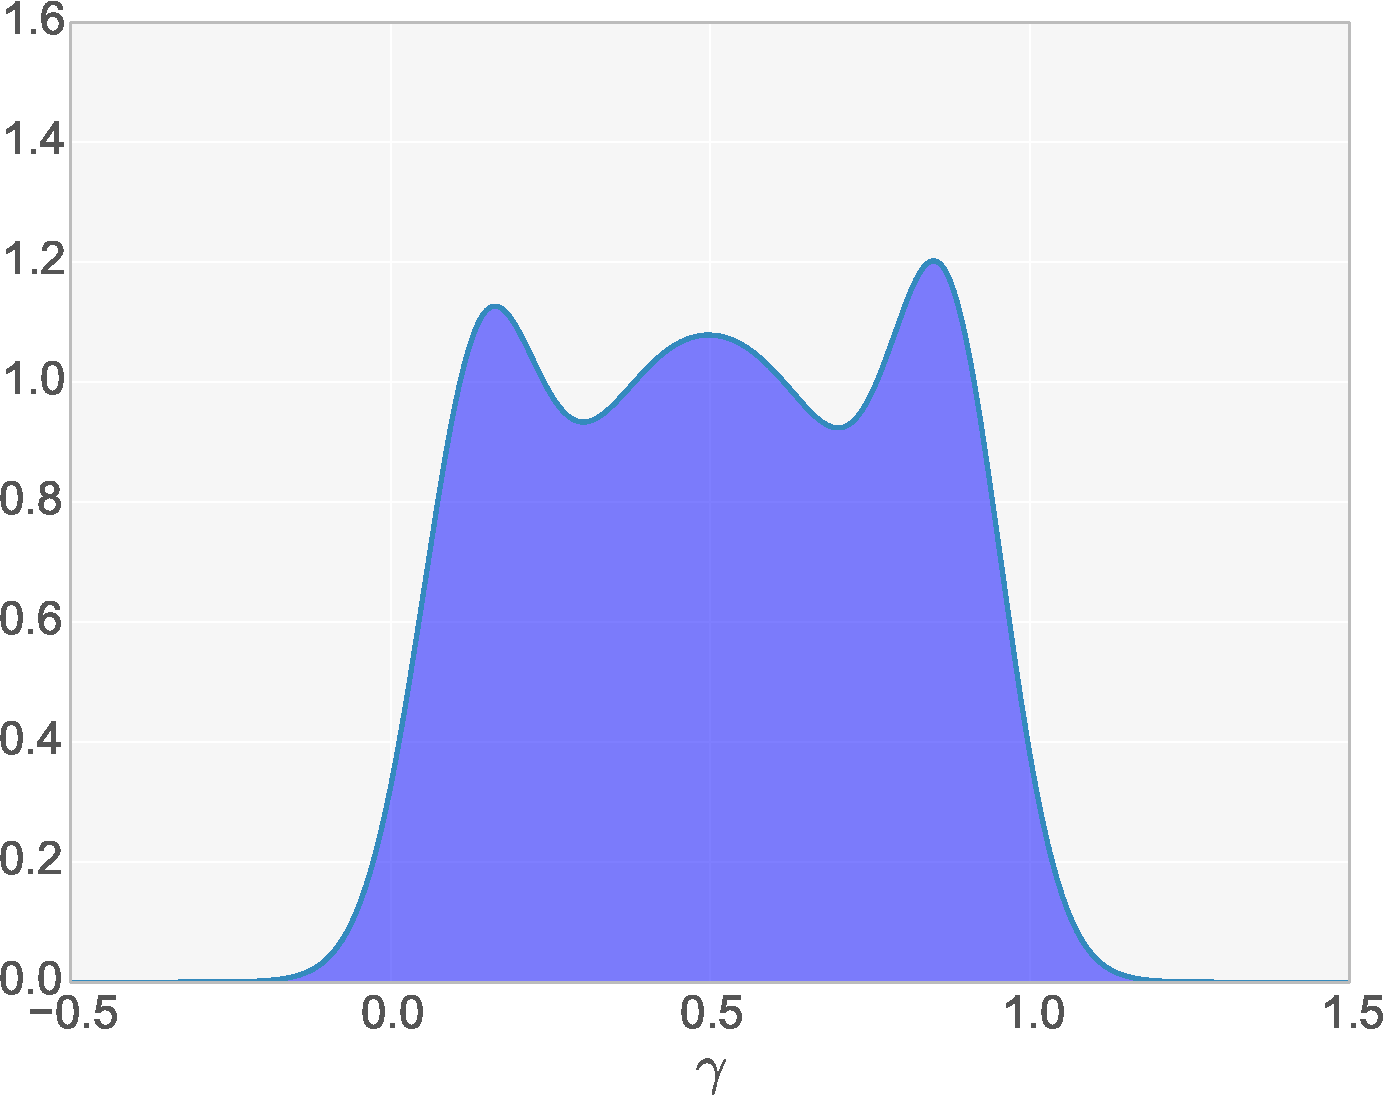
\includegraphics[width=.3\textwidth]{learned1}
	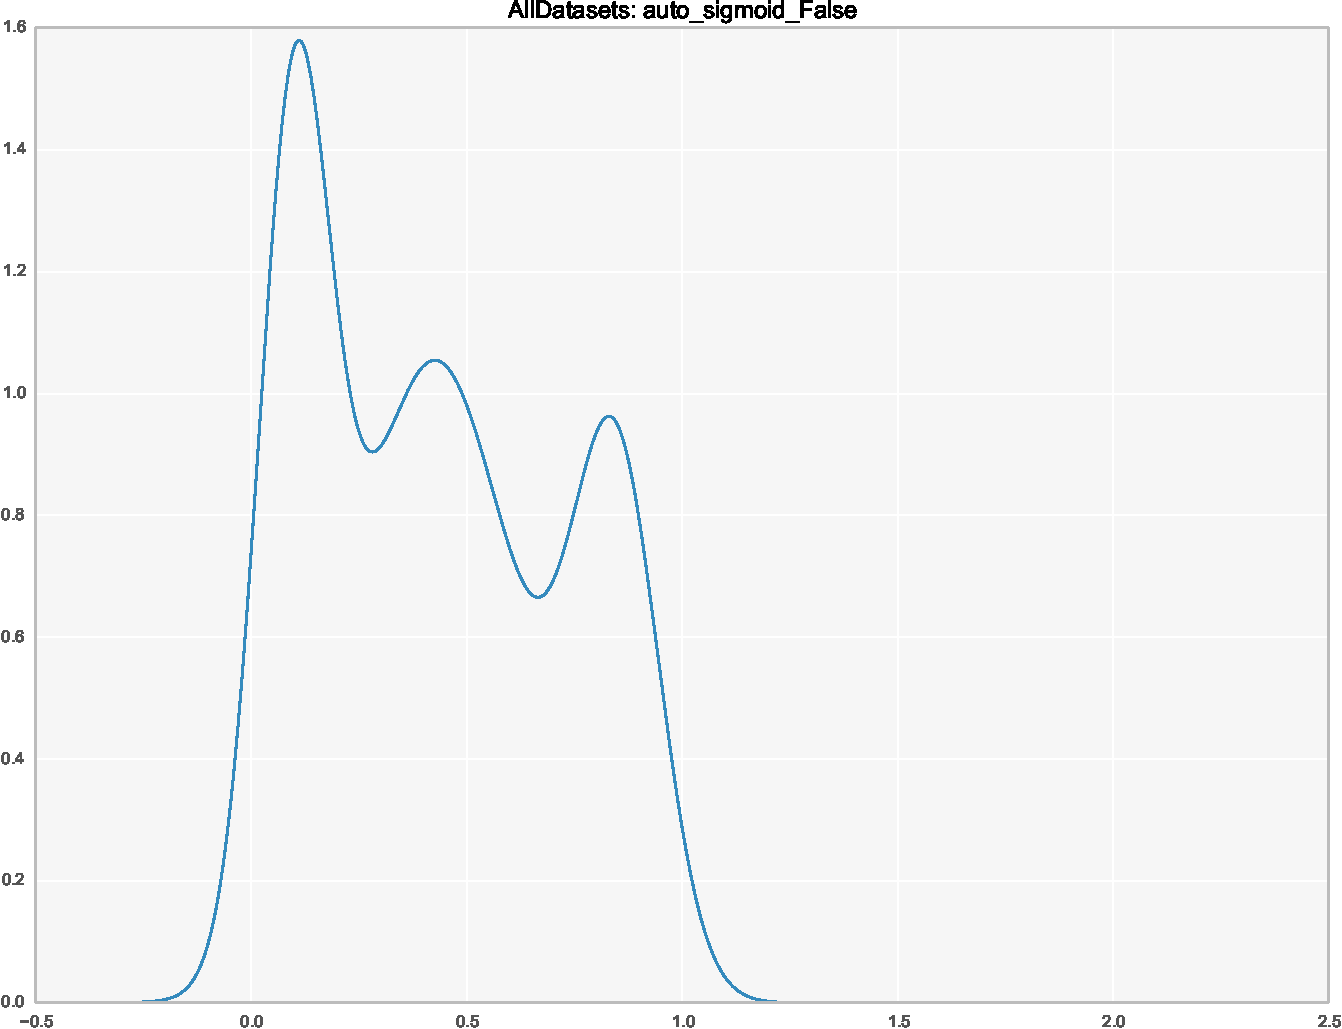
\includegraphics[width=.3\textwidth]{learned2}
	\caption[Uninformative learned general priors]{Distributions of the $\gamma$ hyperparameter learned from the performance indices over
	a large group of datasets. The context gamma for signature auto\_sigmoid\_False} \label{img:learned1}
	\label{fig:learned_gamma1}
\end{figure}


\begin{figure}[h!]
	\centering
	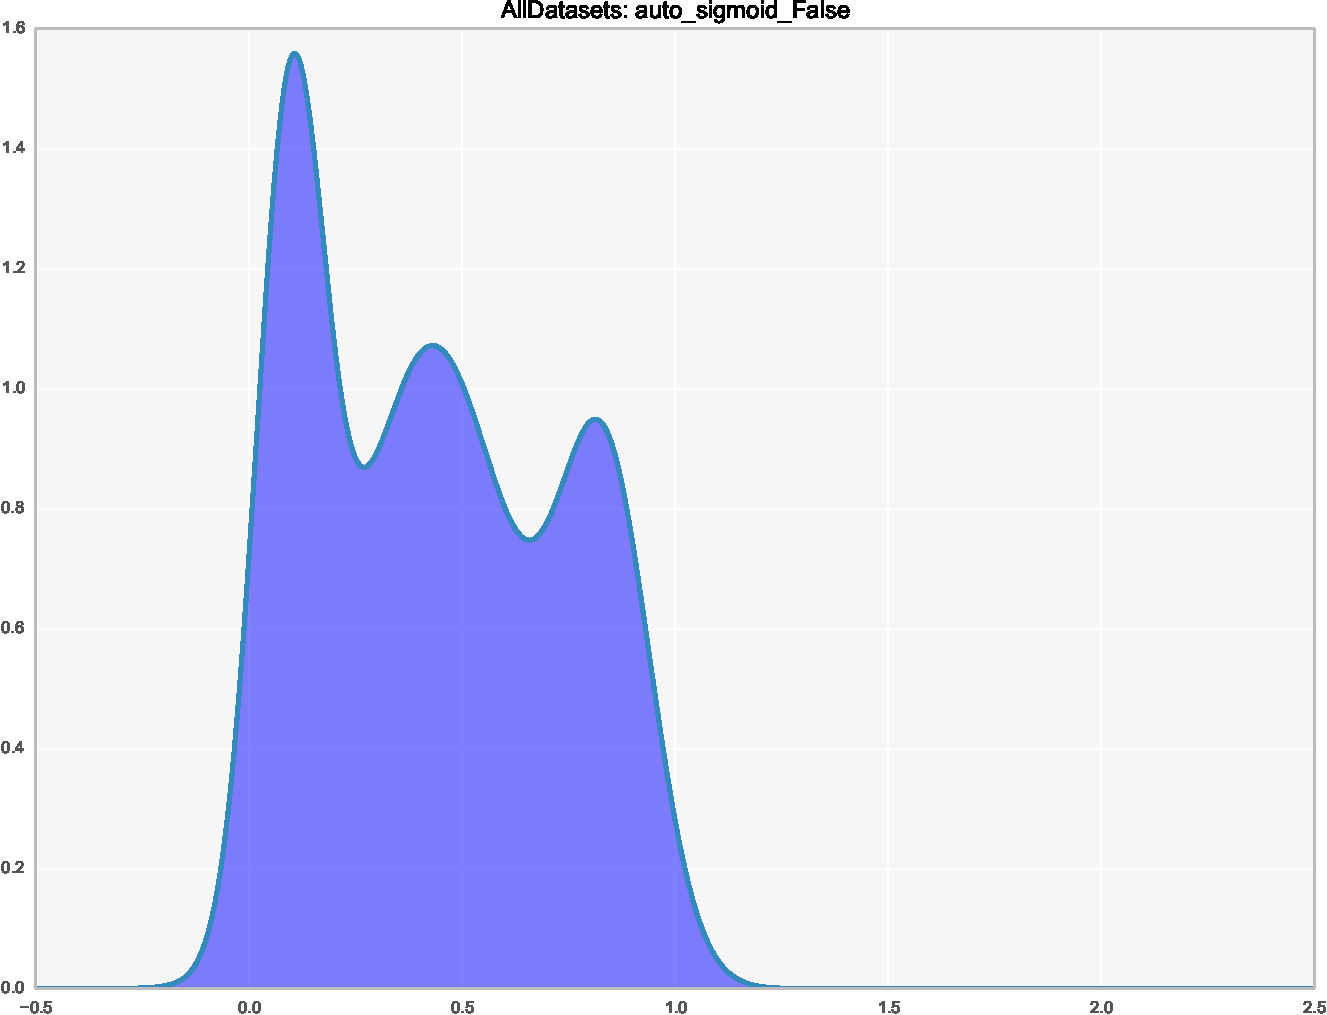
\includegraphics[width=0.3\textwidth]{learned3}
	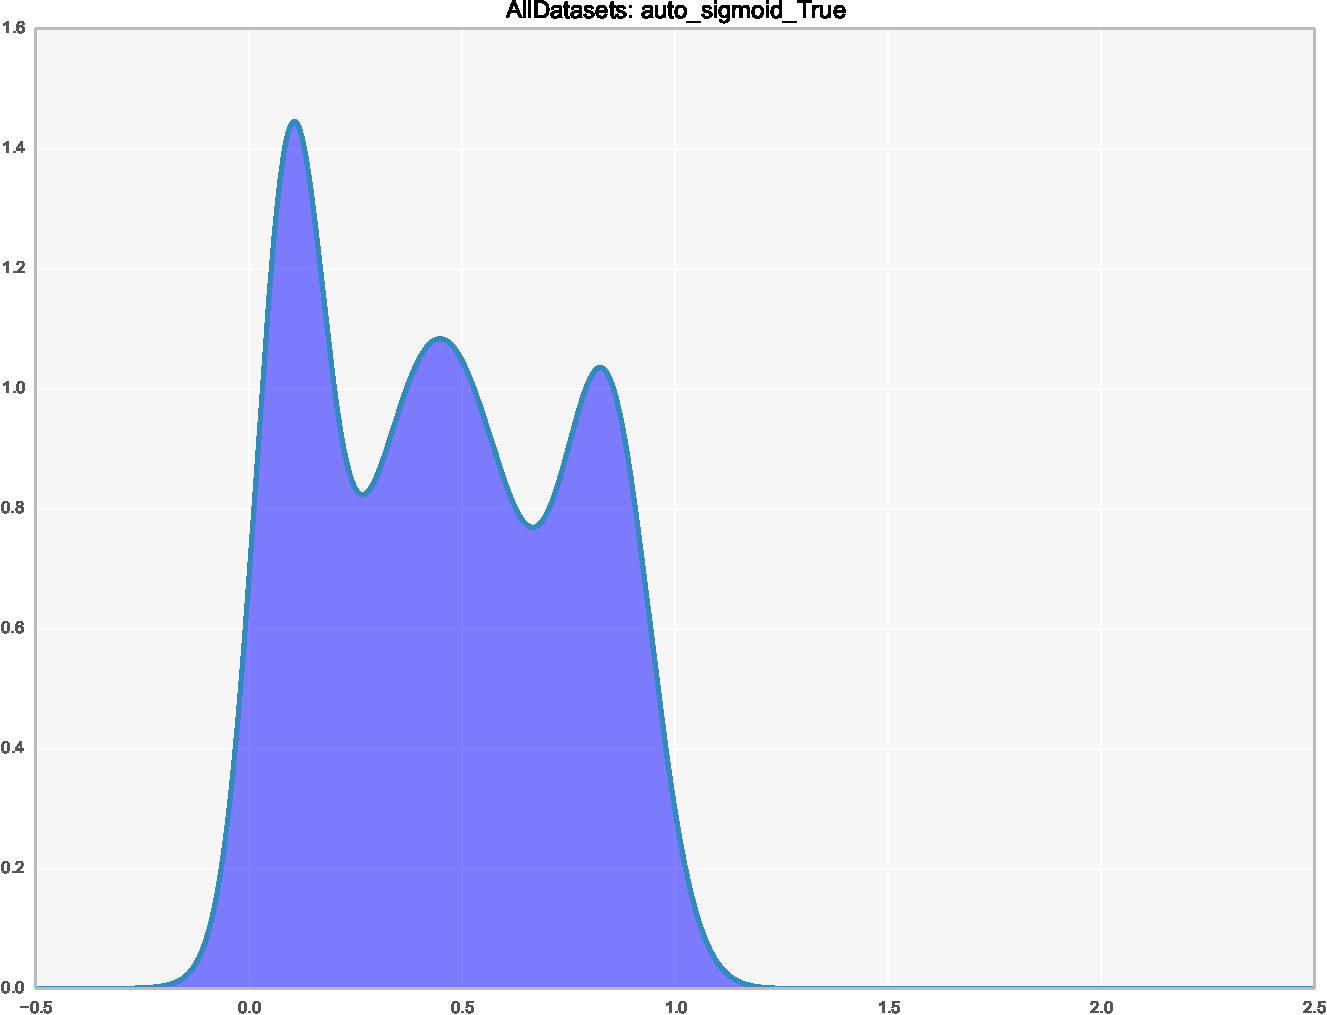
\includegraphics[width=.3\textwidth]{learned4}
	\caption[Informative learned general priors]{gamma for signature auto\_poly\_False}
	\label{fig:learned_gamma2}
\end{figure}

